\let\negmedspace\undefined
\let\negthickspace\undefined
\documentclass[journal]{IEEEtran}
\usepackage[a5paper, margin=10mm, onecolumn]{geometry}
%\usepackage{lmodern} % Ensure lmodern is loaded for pdflatex
\usepackage{tfrupee} % Include tfrupee package

\setlength{\headheight}{1cm} % Set the height of the header box
\setlength{\headsep}{0mm}     % Set the distance between the header box and the top of the text

\usepackage{gvv-book}
\usepackage{gvv}
\usepackage{cite}
\usepackage{amsmath,amssymb,amsfonts,amsthm}
\usepackage{algorithmic}
\usepackage{graphicx}
\usepackage{textcomp}
\usepackage{xcolor}
\usepackage{txfonts}
\usepackage{listings}
\usepackage{enumitem}
\usepackage{mathtools}
\usepackage{gensymb}
\usepackage{comment}
\usepackage[breaklinks=true]{hyperref}
\usepackage{tkz-euclide} 
\usepackage{listings}
\usepackage{gvv}                                        
\def\inputGnumericTable{}                                 
\usepackage[latin1]{inputenc}                                
\usepackage{color}                                            
\usepackage{array}                                            
\usepackage{longtable}                                       
\usepackage{calc}                                             
\usepackage{multirow}                                         
\usepackage{hhline}                                           
\usepackage{ifthen}                                           
\usepackage{lscape}
\usepackage{circuitikz}
\tikzstyle{block} = [rectangle, draw, fill=blue!20, 
    text width=4em, text centered, rounded corners, minimum height=3em]
\tikzstyle{sum} = [draw, fill=blue!10, circle, minimum size=1cm, node distance=1.5cm]
\tikzstyle{input} = [coordinate]
\tikzstyle{output} = [coordinate]

\begin{document}


\bibliographystyle{IEEEtran}
\vspace{3cm}

\title{4.3.39}
\author{EE25BTECH11049 - Sai Krishna Bakki}
 \maketitle
% \newpage
% \bigskip
{\let\newpage\relax\maketitle}

\renewcommand{\thefigure}{\theenumi}
\renewcommand{\thetable}{\theenumi}
\setlength{\intextsep}{10pt} % Space between text and floats


\numberwithin{equation}{enumi}
\numberwithin{figure}{enumi}
\renewcommand{\thetable}{\theenumi}
\textbf{Question:}\\
If the point (3, 4) lies on the line 3y = ax + 7, find the value of a.\\
\solution\\
Given
\begin{align}
    \vec{P}=\myvec{3\\4},\vec{x}=\myvec{x\\y}\\
    \myvec{a & -3}\vec{x}=-7
\end{align}
Since point (3,4) lies on the line, substitute (0.1) in (0.2),we get
\begin{align}
        \myvec{a & -3}\vec{P}=-7\\
        \myvec{a & -3}\myvec{3\\4}=-7\ \\
        3a-12=-7\implies a=\frac{5}{3}
\end{align}
$\therefore$ The value of a is \textbf{$\frac{5}{3}$}.
\newpage
 \begin{figure}
    \centering
    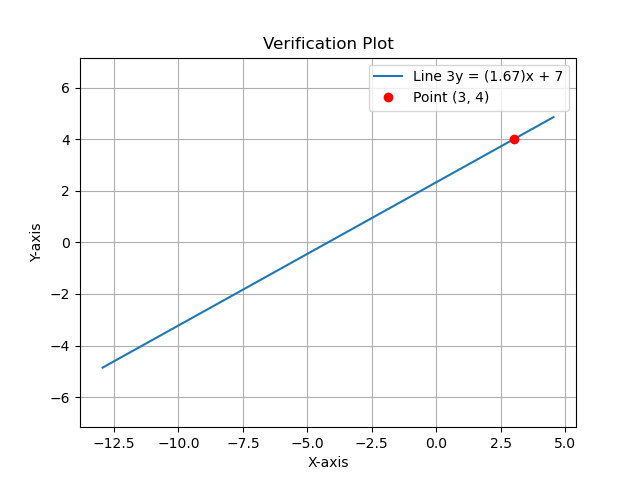
\includegraphics[width=0.9\columnwidth]{figs/Figure_1.png}
    \label{fig:placeholder}
    \caption{}
\end{figure}
\end{document}